In this chapter, the results of numerical simulations for 
blood flow in a coronary artery are presented. 
The lumen radius of the coronary artery used was $R=0.0015m$, 
the viscosity used was $\mu=0.0035Pa.s$ and the specific gravity used was
$\rho=1060kg/m^3$ as suggested by Bozsak, Chomaz and Barakat (2014)
 \cite{bozsak2014}. According to Kessler et al. (1998) 
\cite{kessler1998}, the blood velocity in the coronary artery 
is $u=12cm/s$. Thus, the Reynolds number used will be 
$Re=54.5$. 

\par 
The Navier-Stokes equation is used according to the 
vorticity-streamfunction formulation with 
the species transport equation for four geometries proposed 
by Wang et al. (2017) \cite{wang2017}, however modified to 
cartesian coordinates as shown in \ref{coronary artery geo}. 
In the \ref{canal curvado} section, the coronary artery 
with atherosclerosis is modeled as a flow in a curved channel. 
In the section \ref{canal curvado com stent}, the numerical 
simulation for the coronary artery with atherosclerosis 
and a drug-eluting stent is presented for several 
\textit{Schmidt} number, such as $Sc=1$ and $10$. 
In the \ref{canal real} section, a numerical simulation 
of a real coronary artery with atherosclerosis is presented 
and in the \ref{canal real com stent}, the real coronary 
artery with atherosclerosis and a drug-eluting stent is 
simulated with several numbers of \textit{Schmidt} number 
as in the case of the section \ref{canal curvado com stent}. 
Due to symmetry, only half of the domain was simulated. 
The simulation was visualized using the \textit{Paraview} open-source 
software proposed by Henderson (2007) \cite{paraview}.


\begin{figure}[H]
     \centering
     \begin{minipage}{.45\linewidth}
      \centering
      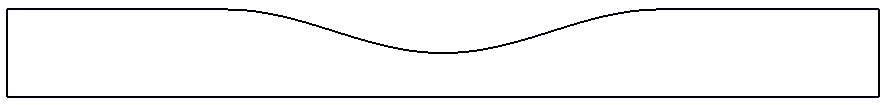
\includegraphics[scale=0.22]{./02_chaps/cap_solution/figure/Curved.png}\\
      (a)
     \end{minipage}%
     \begin{minipage}{.45\linewidth}
      \centering
      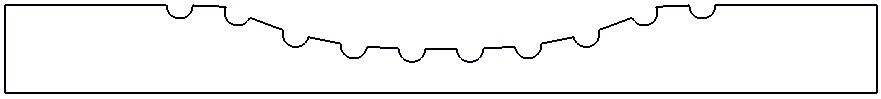
\includegraphics[scale=0.22]{./02_chaps/cap_solution/figure/CurvedStrut.png}\\
      (b)
     \end{minipage}
     \begin{minipage}{.45\linewidth}
      \centering
      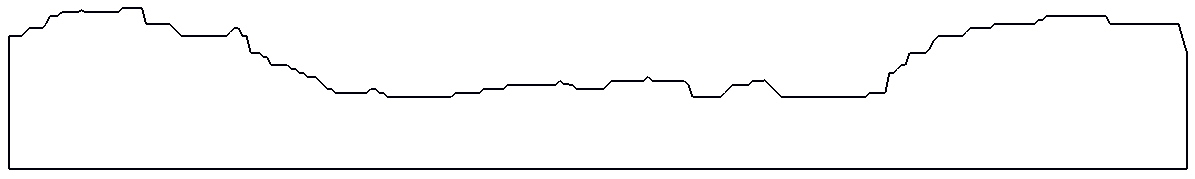
\includegraphics[scale=0.16]{./02_chaps/cap_solution/figure/Real.png}\\
      (c)
     \end{minipage}%
     \begin{minipage}{.45\linewidth}
      \centering
      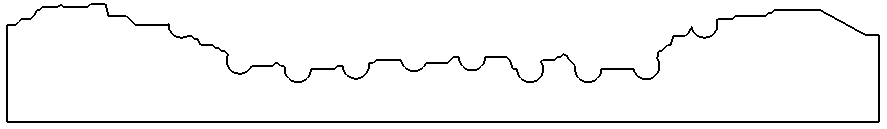
\includegraphics[scale=0.22]{./02_chaps/cap_solution/figure/RealStrut.png}\\
      (d)
     \end{minipage}
     \medskip
     \caption{Non-dimensional Domaian for blood flow in coronary artery
     The radius used was $R=1$ and and the lumen length was $L=10R$.
     (a) Curved Channel
     (b) Curved Channel with Drug-Eluting Stent
     (c) Real Channel
     (d) Real Channel with Drug-Eluting Stent.}
     \label{coronary artery geo}
\end{figure}
